\section{Full ETT prequential results}
\label{app:ett}

\begin{figure*}[t]
  \centering
  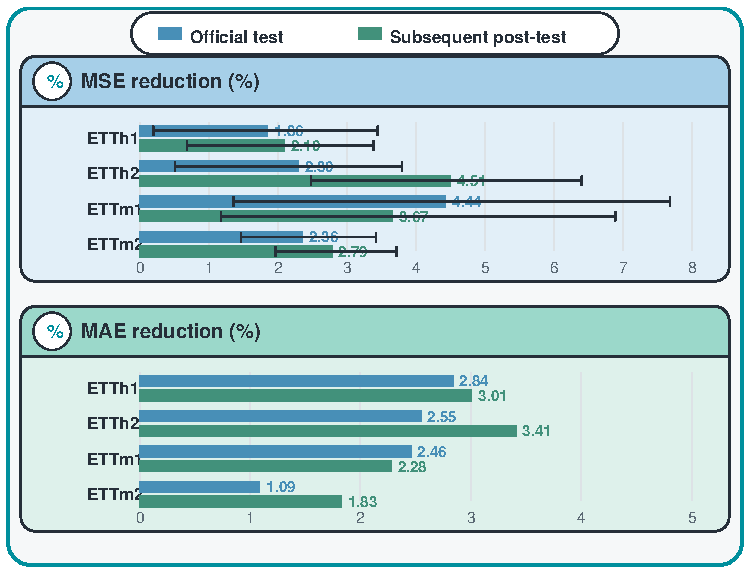
\includegraphics[width=0.65\textwidth]{figures/ett_gains.pdf}
  \caption{Pooled MSE and MAE reductions over matched TimeMixer forecasts
  across three seeds. The post-test timeline is chronologically subsequent to
  the standard split and is excluded from model and correction selection.
  Horizontal lines on MSE bars are 95\% paired moving-block-bootstrap
  intervals. Higher is better.}
  \label{fig:ett-gains}
\end{figure*}

\begin{table*}[h]
\centering
\small
\caption{Pooled MSE reductions and 95\% paired moving-block-bootstrap
intervals. Intervals are candidate-minus-baseline MSE, so values below zero
favor \method{}.}
\label{tab:ett-confidence}
\begin{tabular}{lrrrr}
\toprule
& \multicolumn{2}{c}{Official test} &
\multicolumn{2}{c}{Subsequent post-test}\\
\cmidrule(lr){2-3}\cmidrule(lr){4-5}
Dataset & Reduction & 95\% interval & Reduction & 95\% interval\\
\midrule
ETTh1 & 1.86\% & $[-0.013169,-0.000768]$ &
2.10\% & $[-0.017964,-0.003646]$\\
ETTh2 & 2.30\% & $[-0.011055,-0.001485]$ &
4.51\% & $[-0.011830,-0.004583]$\\
ETTm1 & 4.44\% & $[-0.024903,-0.004411]$ &
3.67\% & $[-0.034576,-0.005918]$\\
ETTm2 & 2.36\% & $[-0.006030,-0.002587]$ &
2.79\% & $[-0.004747,-0.002511]$\\
\bottomrule
\end{tabular}
\end{table*}

\begin{table*}[h]
\centering
\small
\setlength{\tabcolsep}{4pt}
\caption{Per-seed MSE reductions (\%) for the ETT prequential
study. All corresponding MAE values also improve.}
\label{tab:ett-seeds}
\begin{tabular}{lrrrrrr}
\toprule
& \multicolumn{3}{c}{Official test} &
\multicolumn{3}{c}{Subsequent post-test}\\
\cmidrule(lr){2-4}\cmidrule(lr){5-7}
Dataset & 2021 & 2022 & 2023 & 2021 & 2022 & 2023\\
\midrule
ETTh1 & 1.59 & 1.49 & 2.48 & 2.39 & 2.08 & 1.84\\
ETTh2 & 4.31 & 1.18 & 1.37 & 6.29 & 3.69 & 3.49\\
ETTm1 & 2.72 & 8.35 & 2.06 & 2.12 & 5.50 & 3.39\\
ETTm2 & 2.36 & 2.54 & 2.17 & 2.62 & 2.72 & 3.02\\
\bottomrule
\end{tabular}
\end{table*}

The intervals use 5,000 moving-block bootstrap resamples of length 96 after
averaging aligned seed losses at each origin. The later timeline begins on
2018-02-21 for ETTh and ends on 2018-06-25 for ETTm. ETTh uses the fixed stack
specified in the experiment protocol; ETTm retrieval adds an official-test
residual only after its target interval has elapsed.
